
\chapter{Diseño}

% Arquitectura del software, diagramas de clases, diagramas de secuencia

\section{Arquitectura del software}

En esta sección muestro un esquema que representa la arquitectura general del software mediante el diagrama de paquetes. Dicho diagrama puede verse en la figura \ref{paquetes}.\newline


\begin{figure}[h]
	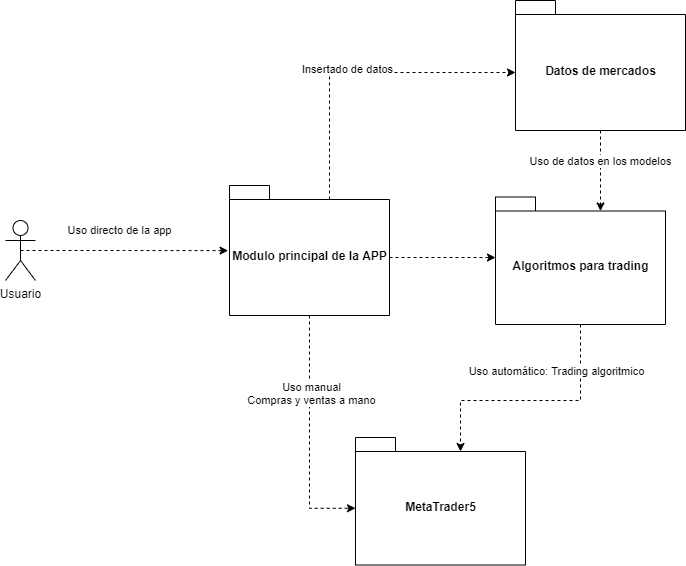
\includegraphics[width=1.1\textwidth]{imagenes/arquitectura general.png}
	\caption{Arquitectura general del software.} \label{paquetes}
\end{figure}


Como resumen, en el esquema podemos ver cuál es la estructura principal del proyecto. El usuario de la aplicación (véase punto \ref{implicados}, segundo implicado) será el que haga un uso directo de la interfaz de la aplicación. El administrador (primer implicado, \ref{implicados}) sólo interviene en la gestión de usuarios, incluida dentro del módulo principal de la APP. A continuación presento cada uno de los módulos con sus funciones y demás utilidades:

\begin{itemize}
	\item \textbf{Interfaz principal de la APP}: este módulo se corresponde con el controlador principal del software. Es usado por el usuario a través de una interfaz escrita en \textit{Django} y se comunicará con el resto de módulos directamente.
	\item \textbf{Gestión de usuarios}: módulo proporcionado por \textit{Django} por defecto. Implementa la página \textit{admin} y las posibilidades de añadir nuevos usuarios, eliminarlos, editarlos, etc. 
	\item \textbf{Datos de mercados}: este módulo se corresponderá con la base de datos y las operaciones que hagamos con dichos datos (insertado de datos, adaptaciones a cada algoritmo, etc.) Será usado por la interfaz principal de la aplicación y mandará los \textit{inputs} a los algoritmos.
	\item \textbf{Algoritmos de trading o backend}: se corresponde con el backend o código fuente de la aplicación. Aquí se encontrará cada uno de los algoritmos que usemos para trading algorítmico. Recibe datos de la BBDD y se comunica con el módulo de la plataforma comercial para indicar cada una de las operaciones decididas y obtener información en tiempo real. Se comunica con la interfaz principal para devolver los resultados de las opciones de operar y/o backtesting.
	\item \textbf{Plataforma comercial}: Módulo externo de la aplicación, se usa para mandar órdenes de operaciones y recibir resultados e información en tiempo real.
\end{itemize}

\section{Cuestiones más relevantes: algoritmos de trading y gestión de datos de mercado}

En este apartado comento el diseño de dos de las cuestiones más relevantes de la aplicación: los algoritmos de trading y la gestión de datos de mercado.\newline

En cuanto al \textbf{módulo de algoritmos de trading}, se creará un modelo referente a cada uno de los algoritmos o estrategias para operar. Se implementará aquí el método de Wyckoff, mencionado en el contexto teórico del proyecto. El método de Wyckoff será uno de los objetos de este modelo. Cada uno de los objetos o algoritmos, serán como cajas negras. El usuario podrá utilizar cada uno de ellos sin saber ni tener que saber cómo funcionan.\newline

Por el diseño de la aplicación, el módulo de algoritmos de trading es un módulo totalmente independiente de los demás. Esto puede verse en la figura \ref{paquetes}, arquitectura general. Que sea independiente de los demás quiere decir que en el mismo módulo se desarrollan los algoritmos. El procesado de datos, inputs y outputs es trabajo del resto de módulos. A cada estrategia le llegarán siempre unos datos de entrada, y dará unos datos de salida. En este caso, la entrada serán los datos históricos del mercado en el que queremos operar en cada caso; y la salida, las operaciones realizadas y balance obtenido.\newline

En segundo lugar, tenemos el módulo de gestión de datos de mercado.\newline

El usuario a través de las vistas de la APP, podrá elegir qué mercado financiero guardar en su base de datos y los parámetros a elegir: temporalidad, fecha inicio, etc. Los datos de los mercados financieros seguirán el formato \textit{OHLC} y serán usados por el módulo de trading o algoritmos de trading; y por la interfaz para la visualización de datos antiguos.\newline

Los datos que el usuario guarda serán recogidos a través de la plataforma comercial usada, \textit{MetaTrader5}. Los datos guardados serán referentes a cada usuario, lo que quiere decir que otro usuario cualquiera de la aplicación tendrá que guardar los suyos propios ya que no tendrá acceso a los de los demás.\newline

Las dos cuestiones presentadas en este punto: algoritmos y gestión de datos; serán explicadas de manera más técnica y desarrollada en la parte de implementación del proyecto.\newline



\section{Diseño de clases}

En esta sección se muestra el diagrama de clases del proyecto. Este diagrama se puede ver en la figura \ref{diagrama_clases} \newline

Las clases \textit{AbstractUser} y \textit{User} forman parte del modelo \textit{auth} de \textit{Django} y proporcionan los objetos que se corresponderán con los usuarios de la APP. He relacionado esta clase \textit{User} con una clase personalizada \textit{Sesion}, que es instanciada a la vez que se instancia \textit{User}, de manera automática. Por otra parte, \textit{ManagementUtility} es la clase que arranca el servidor web de \textit{Django}.\newline

\textit{AlgoritmoTrading}, \textit{Mercado} y \textit{WyckoffTrading} son otras clases personalizadas encargadas de instanciar los distintos algoritmos de trading, los mercados de los que vamos a obtener información y el método de trading de Wyckoff a aplicar, respectivamente. \newline

En el caso de WyckoffTrading, la clase es instanciada cuando operamos en tiempo real o backtesting con el algoritmo de trading. Es por ello que esta clase se usa puramente para desarrollo y no es un modelo, a diferencia de las demás que sí son modelos de Django.\newline

\begin{figure}[h]
	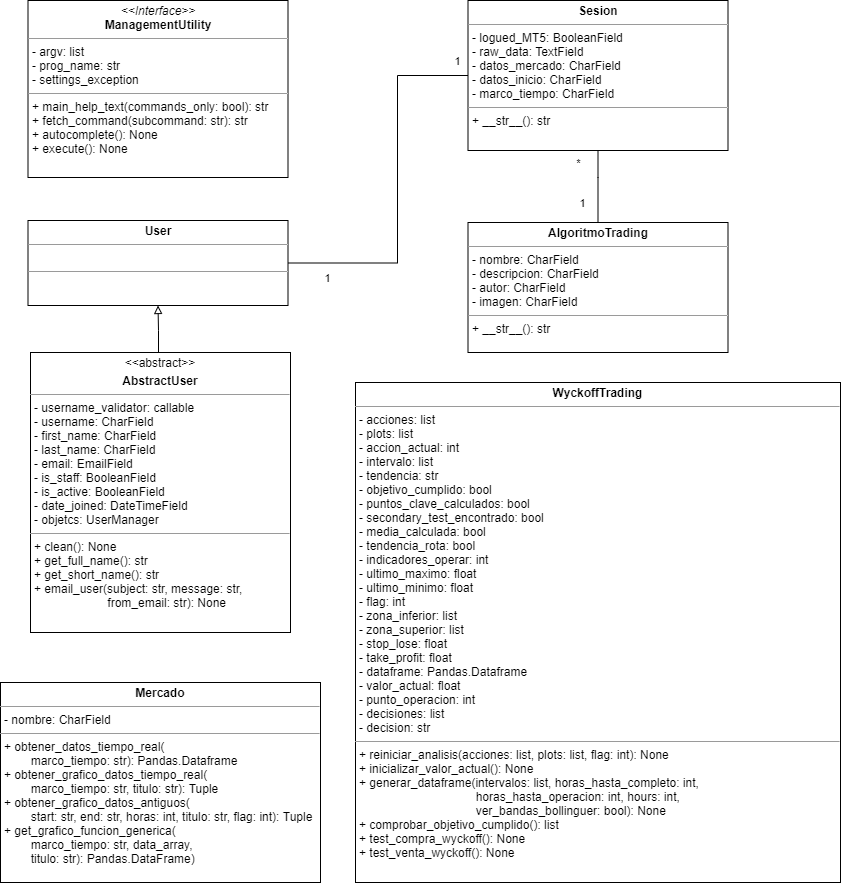
\includegraphics[width=1.2\textwidth]{imagenes/diagrama_clases.png}
	\caption{Diagrama de clases de la APP} \label{diagrama_clases}
\end{figure}

\section{Diagramas de secuencia}

En este apartado incluyo los diagramas de secuencia referentes a las distintas funcionalidades de la aplicación. Las partes del sistema referentes a vistas se han marcado con cuadros de color azul; las partes referentes a los controladores se han marcado con color azul más claro; y los modelos están señalados en gris. El objetivo de esta diferenciación es dejar claro qué cosa representa cada una de las partes del patrón de arquitectura \textit{Modelo-Vista-Controlador}. \newline

En la imagen \ref{iniciar_app} se ven los pasos realizados para iniciar la aplicación. \newline

\begin{figure}[h] 
	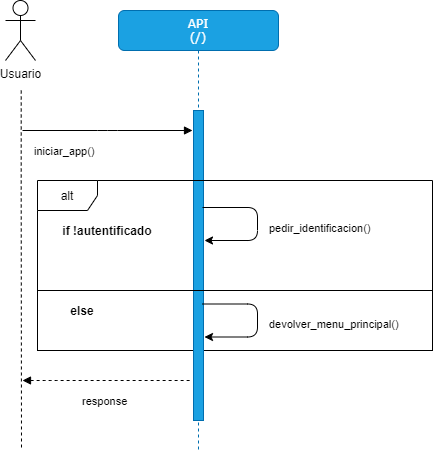
\includegraphics[width=0.6\textwidth]{imagenes/diagramas_secuencia/iniciar_app.png}
	\caption{Diagrama de secuencia de inicio de la APP} \label{iniciar_app}
\end{figure}

En la figura \ref{secuencia_crear_usuario} se pueden ver los pasos realizados por el sistema para crear un usuario y cómo lo enriquece con los detalles específicos de la sesión. \newline

\begin{figure}[h] 
	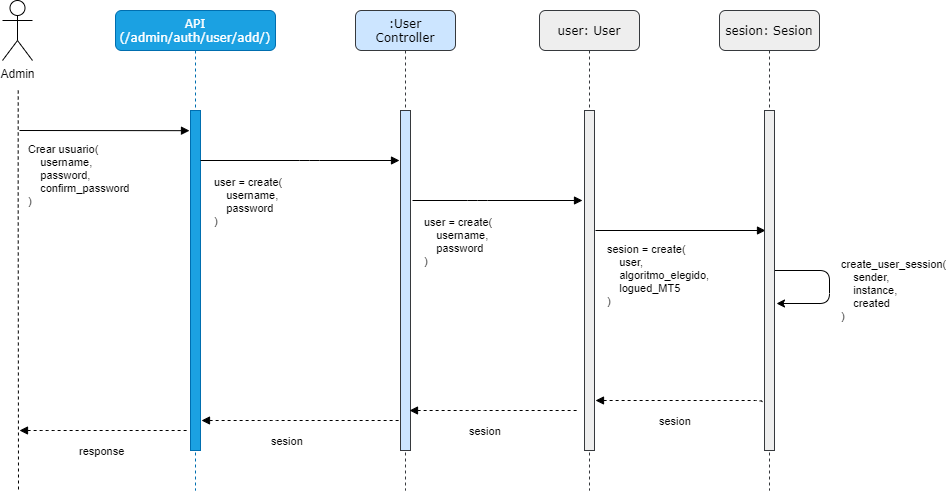
\includegraphics[width=1.2\textwidth]{imagenes/diagramas_secuencia/gestion_usuarios.png}
	\caption{Diagrama de secuencia de la creación de usuarios} \label{secuencia_crear_usuario}
\end{figure}

En el diagrama \ref{login_logout} se sigue el comportamiento de la aplicación cuando el usuario se identifica o cierra sesión en la APP. \newline

\begin{figure}[h] 
	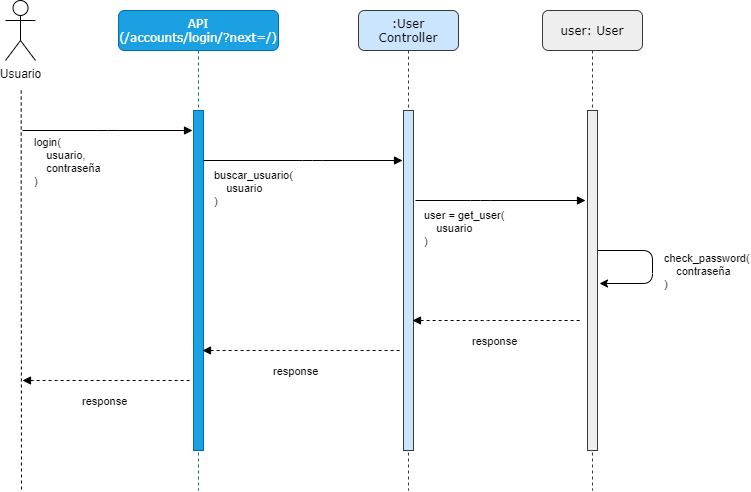
\includegraphics[width=1\textwidth]{imagenes/diagramas_secuencia/login_logout.png}
	\caption{Diagrama de secuencia de login y logout de usuarios} \label{login_logout}
\end{figure}

En la figura \ref{login_logout_MT5} se representan los pasos de la aplicación al identificarse y cerrar sesión en el bróker de MetaTrader5.\newline

\begin{figure}[h] 
	\includegraphics[width=1.1\textwidth]{imagenes/diagramas_secuencia/login_logout_mt5.png}
	\caption{Diagrama de secuencia de login y logout de usuarios en el bróker en MetaTrader5} \label{login_logout_MT5}
\end{figure}

En el diagrama \ref{gestion_datos} se representan los pasos de la aplicación realizados cuando un usuario guarda los datos de mercados en la database, por medio de la APP.\newline

\begin{figure}[h] 
	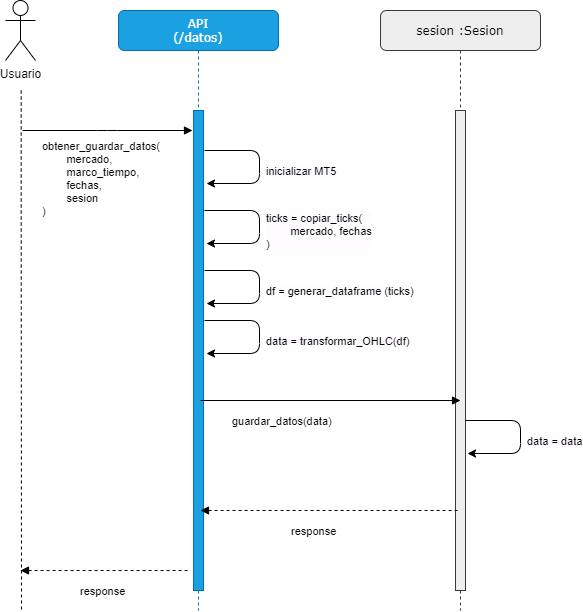
\includegraphics[width=1.1\textwidth]{imagenes/diagramas_secuencia/gestion_datos.png}
	\caption{Diagrama de secuencia gestión de datos} \label{gestion_datos}
\end{figure}

En la imagen \ref{ver_datos_secuencia} se muestran los pasos de la aplicación para las funcionalidades de visualización de datos antiguos o en tiempo real.\newline

\begin{figure}[h] 
	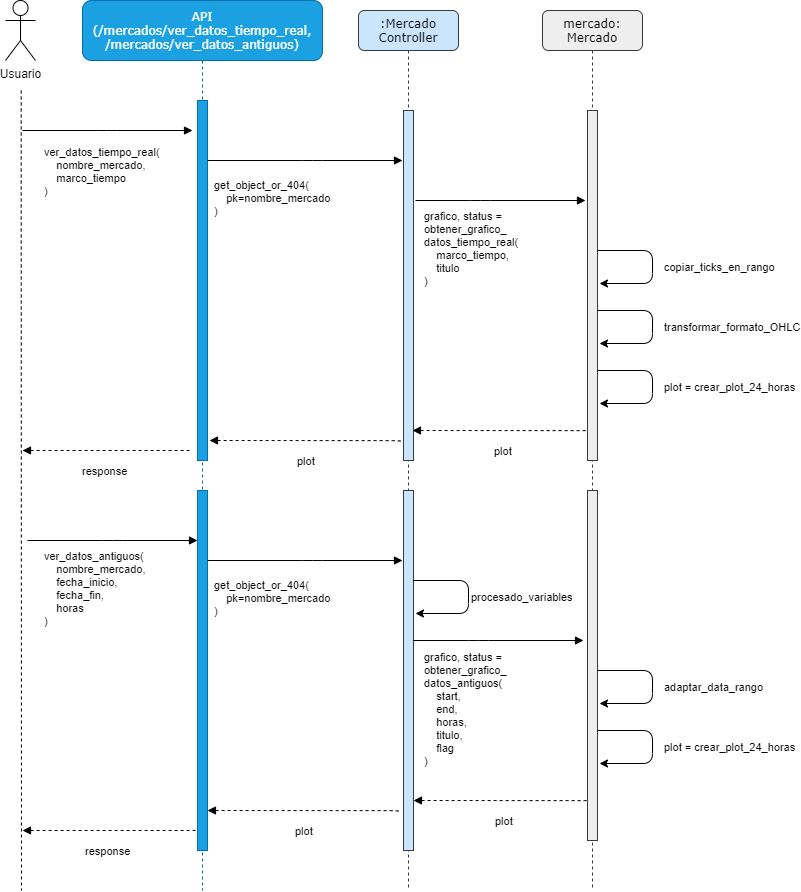
\includegraphics[width=1.1\textwidth]{imagenes/diagramas_secuencia/ver_datos.png}
	\caption{Diagrama de secuencia de visualización de datos antiguos y en tiempo real} \label{ver_datos_secuencia}
\end{figure}

Por último, en la figura \ref{algoritmos_secuencia} se muestran los pasos de la aplicación para la elección de estrategias de trading y trading algorítmico y backtesting.\newline

\begin{figure}[h] 
	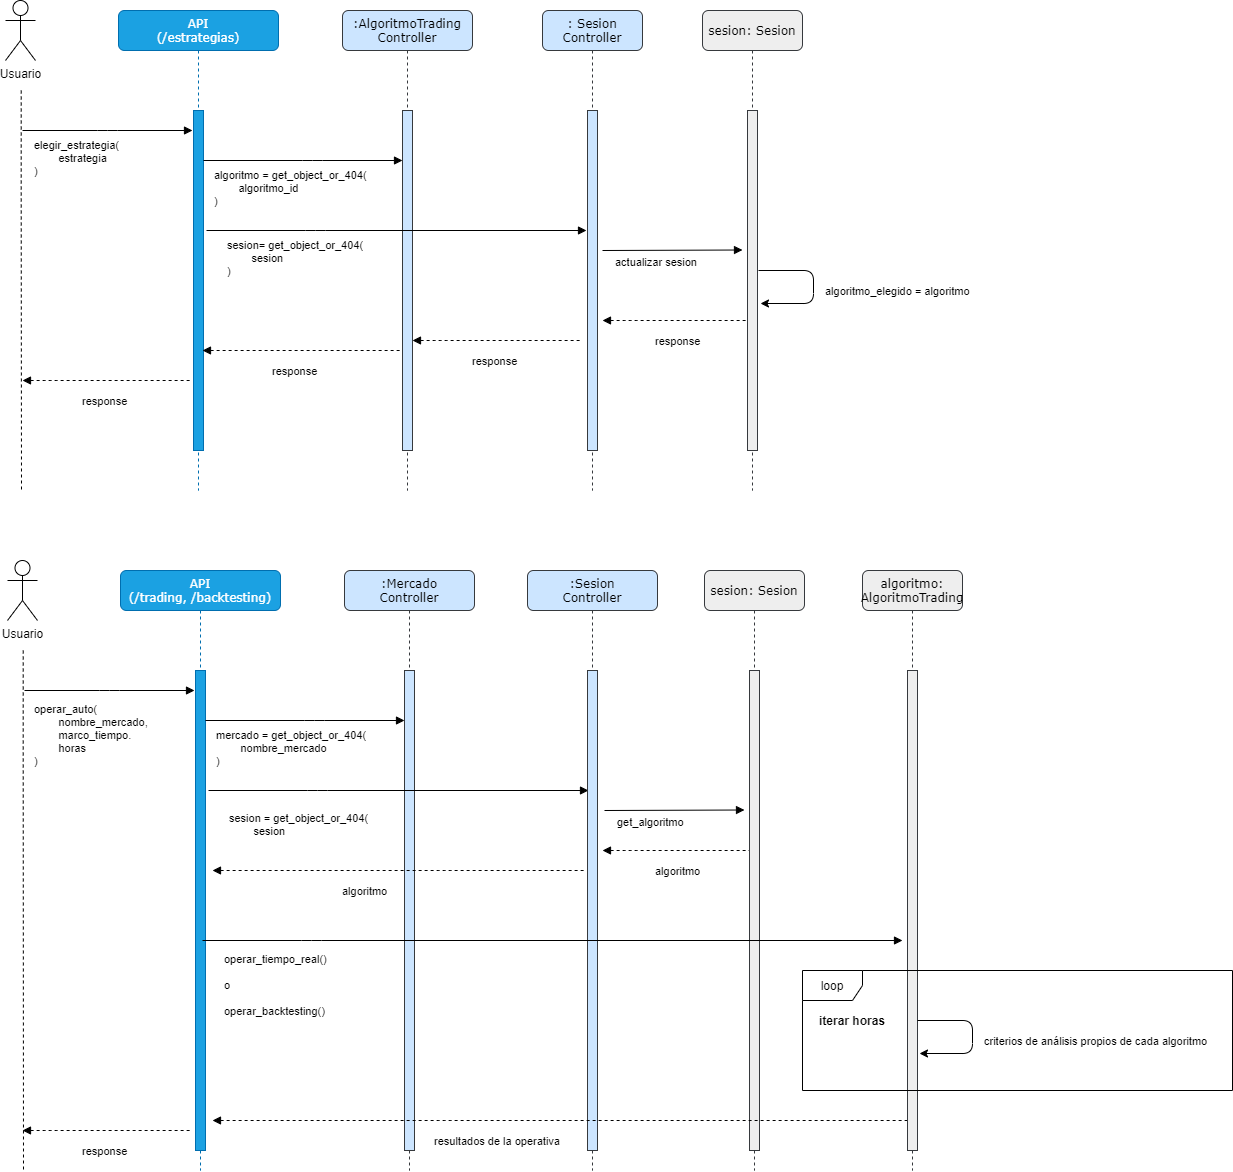
\includegraphics[width=1.35\textwidth]{imagenes/diagramas_secuencia/algoritmos_secuencia.png}
	\caption{Diagrama de secuencia de elección de algoritmos y trading automático y backtesting} \label{algoritmos_secuencia}
\end{figure}

\section{Primer diseño de la interfaz} \label{primer_diseño}

La página web principal mostrará un menú con distintos botones que implementan funcionalidades diferentes. Previo a este menú tendremos un formulario para identificarnos como usuarios de la aplicación. A ambos lados del menú principal y durante todas las vistas de la APP tendremos hiperenlaces con accesos directos a distintas funcionalidades de la aplicación. A continuación muestro una serie de borradores con diseños de cada una de las secciones de la interfaz.\newline

En este primer diseño que muestro en la siguiente imagen, se puede ver el menú principal de la aplicación.\newline

\begin{figure}[h] 
	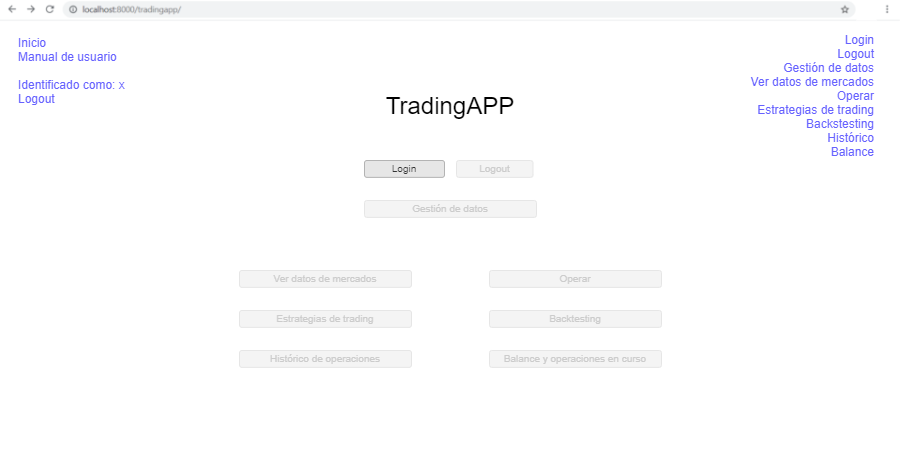
\includegraphics[width=1.2\textwidth]{imagenes/menu_principal.png}
	\caption{Primer diseño del menú principal de la APP} \label{menu_principal}
\end{figure}

En la imagen mostrada vemos los siguientes botones: \textit{Login}, \textit{Logout}, \textit{Gestión de datos}, \textit{Ver datos de mercados}, \textit{Operar}, \textit{Estrategias de trading}, \textit{Backtesting}, \textit{Histórico de operaciones} y \textit{Balance y operaciones en curso}. En los puntos siguientes explico qué realizaría cada botón y con qué parte del software conectaría.\newline

\begin{itemize}
	\item \textbf{Login}: permite conectar a nuestra cuenta del bróker que usemos en la plataforma comercial, comercial o demo. Véase la siguiente figura. \textit{\textbf{Referencia}: login, RF-2.1.}
	\item \textbf{Logout}: permite cerrar la sesión iniciada anteriormente con el menú de Login. Este botón no estará habilitado hasta que hayamos iniciado sesión. \textit{\textbf{Referencia}: login, RF-2.1.}
	\item \textbf{Gestión de datos}: permite el insertado y procesado de datos de mercado. El usuario podrá a través del menú correspondiente introducir datos al módulo que se encarga de gestionar la BBDD, que son recogidos automáticamente de las bases de datos de la plataforma comercial. \textit{\textbf{Referencia}: procesado de datos}
	\item \textbf{Ver datos de mercados}: permite ver datos de precios de un mercado elegido. Se permite ver datos en un marco de tiempo específico, en rango y de mercados específicos. \textit{\textbf{Referencia}: visualización de datos, RF-3.}
	\item \textbf{Operar}: lleva al usuario a un menú donde podrá operar o usando trading algorítmico. \textit{\textbf{Referencia}: trading algorítmico, RF-4.} 
	\item \textbf{Estrategias de trading}: lleva a un menú en el que se puede obtener información de cada una de las estrategias de trading así como elegir una para que sea usada en las próximas operaciones. \textit{\textbf{Referencia}: trading algorítmico, RF-4.} 
	\item \textbf{Backtesting}: menú similar a Operar. En este caso el usuario podrá iniciar operaciones usando trading algorítmico a partir de una fecha anterior a la actual, simulando el transcurso del tiempo. \textit{\textbf{Referencia}: backtesting, RF-5.} 
	\item \textbf{Histórico de operaciones}: permite al usuario ver un resumen del histórico de operaciones realizadas. \textit{\textbf{Referencia}: información de operaciones, RF-2.3.} 
	\item \textbf{Balance y operaciones en curso}: permite al usuario ver el capital disponible, así como un balance a tiempo real de pérdidas y ganancias y el resumen de las operaciones en curso. \textit{\textbf{Referencia}: capital disponible, RF-2.2; información de operaciones, RF-2.3.} 
\end{itemize}

En la figura \ref{login} muestro lo que sería el menú de \textbf{Login}. En este menú se introducirán \textit{Login}, \textit{Contraseña} y \textit{Servidor} para que nuestra aplicación inicie sesión en la cuenta demo o comercial del bróker usado. Podemos ver el diseño del menú en la figura \ref{logued}. \newline

\begin{figure}[h]
	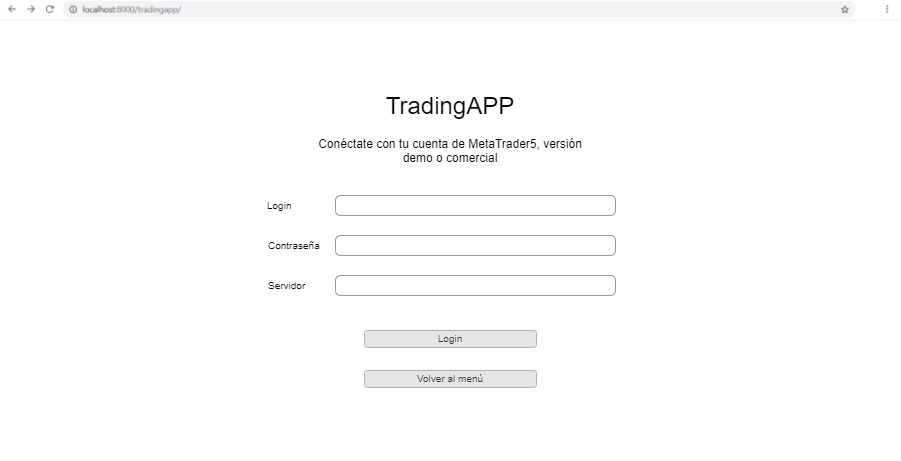
\includegraphics[width=1.2\textwidth]{imagenes/menu_login}
	\caption{Primer diseño del formulario de login en \textit{MT5}} \label{login}
\end{figure}

Una vez estemos conectados en la cuenta proporcionada por el bróker, nuestro menú principal mostrará disponibles las funcionalidades que en la figura \ref{menu_principal} no estaban habilitadas. Dichas funcionalidades dependen directamente de la plataforma comercial o bróker, por lo que necesitan de conexión a la cuenta. \newline

\begin{figure}[h]
	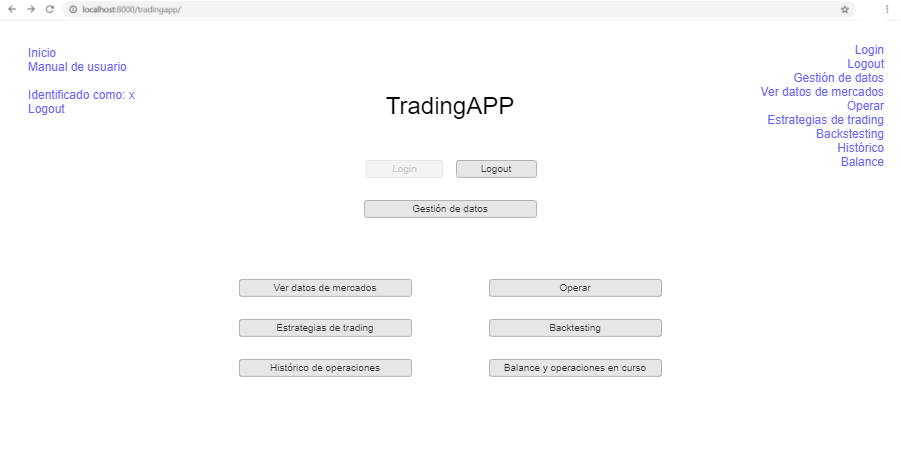
\includegraphics[width=1.2\textwidth]{imagenes/menu_principal_logued.png}
	\caption{Primer diseño del menú principal (usuario identificado en \textit{MT5}) } \label{logued}
\end{figure}



